\chapter{Multirate implementation}
The chapter will describe the three functions which is used in the multirate stages.
\begin{itemize}
\item void downFunc1(int16 dataIn);
\item int16 delayB1(int16 dataIn);
\item int16 upFunc1(int16 dataIn,int16 band);
\end{itemize}
Where downFunc1 is used to decimate and spectral subtract the input sample, delayB1 is used to delay a sample by x samples and upFunc1 is used interpolate the input sample (dataIn) and add the input sample (band) to the interpolated signal. In both downFunc1 and upFunc1 a filter function is used called FIR1 which runs a FIR filter on a data array, which also will be decribed in this chapter. 


\section{Decimation and spectral subtraction implementation}
The decimation block is described in \textbf{XX} and is seen on \autoref{fig:DownsamplingSimulationCopy}.
\begin{figure}[H]
    \centering
	\includegraphics[width=0.7\textwidth, page=2]{Simulation}
    \caption{Decimation block diagram}
    \label{fig:DownsamplingSimulationCopy}
\end{figure}
The block contains different components which has to be implemented:
\begin{itemize}
\item Reading data in.
\item FIR filtering.
\item Spectral subtraction.
\item Downsampling and outputting. 
\end{itemize}
An input sample must be read into a buffer of the size equal to the filter taps. The decimation filter has 51 taps and is described in \autoref{sec:decFilter}, so the buffer must be of equal size, but the buffer can be designed in a number of ways:
\begin{itemize}
\item First in first out (FIFO).
\item Circular
\end{itemize} 
A FIFO buffer is the simple of the two buffer types but it also requires more computation power than a circular buffer. This is because in a FIFO buffer all data must be moved as seen in \autoref{fig:FIFO} while in a circular buffer, see \autoref{fig:Circular}, a pointer can be moved so instead of moving data the pointer moves to the oldest data. So instead of costing the same number of instructions equal to size of the buffer, it only cost the setup of the circular buffer and one instruction per move.   
\begin{figure}[H]
\centering
\begin{subfigure}[t]{0.49\textwidth}
    \centering
	\includegraphics[width=0.6\textwidth]{FIFO.png}
	\label{fig:FIFO}
	\caption{FIFO buffer.}
\end{subfigure}
\begin{subfigure}[t]{0.49\textwidth}
    \centering
	\includegraphics[width=0.4\textwidth]{Circular.png}
	\label{fig:Circular}
	\caption{Circular buffer.}
\end{subfigure}
\caption{Buffer types.}
\label{fig:bufTypes}
\end{figure}
It is choosen to implement a circular buffer because of its cost effectiveness and the implementation is seen on \autoref{ls:ReadingInData}.
\begin{lstlisting}[language={[x86masm]Assembler}, caption = {Reading data in},label={ls:ReadingInData}]
	; "Circular" data in Buffer
	MOV #0, AC0					; Clear AC0
	OR #dataIn1,AC0				; Load address of input data into AC0
	ADD *(#i1),AC0				; Add the addr with the value of the data pointer (Point to oldest data)
	MOV AC0,XAR0				; Move the addr to AR0
	MOV T0, *AR0				; Move the value in T0 to the address
	ADD #1,*(#i1)				; Increment the data pointer
	ADD #1,*(#d1)				; Increment the delay pointer
	CMP *(#i1)==#51,TC1			; Check if the data pointer should reset to 0
	CALLCC resetPtri1, TC1
	CMP *(#d1)==#51,TC1			; Check if the delay pointer should reset to 0
	CALLCC resetPtrd1, TC1
\end{lstlisting}





\section{Interpolation implementation}
The interpolation block is described in \textbf{XX} and is seen on \autoref{fig:upsamplingSimulationCopy}.
\begin{figure}[H]
    \centering
	\includegraphics[width=0.7\textwidth, page=11]{Simulation}
    \caption{Interpolation block diagram}
    \label{fig:upsamplingSimulationCopy}
\end{figure}
The block contains different component which has to be implemented:
\begin{itemize}
\item Reading in data and upsampling.
\item FIR filtering
\item Spectral addition
\end{itemize}


\section{delay implemetation}
The delay block delays a sample x times this is done by implementing a circular buffer with a pointer. The flowchart seen on XX shows the flow of the algorithm.
\todo[inline]{FLOWCHART af delay funktion}
The function uses the following variables:
\begin{itemize}
\item XX
\end{itemize}


\section{FIR filter implementation}